\documentclass[a4paper, 11pt]{article}

\usepackage{graphicx}
\usepackage{tocloft}
\usepackage{xcolor}
\usepackage{hyperref}
\usepackage{amsmath} % for math notation
\usepackage{listings} % for code blocks
\usepackage{graphicx} % for images
\usepackage[T1]{fontenc}
\usepackage[utf8]{inputenc}
\usepackage[german]{babel}
\usepackage{datetime2}
\DTMsetdatestyle{german}

%\settimeformat{ampmtime}
%\setdatetimeformat{dd.~MM.~yyyy}

\lstdefinestyle{code}{
  basicstyle=\fontsize{10pt}{10pt}\selectfont\ttfamily, % set the font
  breaklines=true,      % Automatically break lines
  numbers=left,         % Show line numbers on the left
  language=C++,
  morekeywords={int,double,float,char,bool,void,string,vector,array},
  keywordstyle=\color{blue}\bfseries,
  commentstyle=\color{gray}\ttfamily,
  stringstyle=\color{red}\ttfamily,
}

\begin{document}
\pagenumbering{roman}

\title{Wetterstation}
%\author{}
\date{\today}
\maketitle

\section*{Vorwort}
Hierbei handelt es sich um die Dokumentation zu unserem Microcontrollerprojekt 
im Kurs \textbf{Signalverarbeitung 2} im 3. Semester des Bachelorstudiengangs
Software Engineering.
Die Software befindet sich in unserem öffentlichen Git 
\href{https://github.com/ckiri/wetterstation}{\textcolor{blue}{Repository}}.

\section*{Motivation}
Die Wetterstation soll es ermöglichen Umgebungsmetriken aufzunehmen
und diese dann über einen MQTT Broker zu veröffentlichen.
Das System sendet nur Daten, hört also keinem Topic zu.
Diese Daten können dann z.B. für Smarthome-Anwendungen verwendet
werden.
Folgende Metriken werden aufgezeichnet:
Luftfeuchtigkeit, Luftqualität(Rauch) und Temperatur.
Das System wird auf einem Espressif ESP8266 Mikrocontroller
realisiert.

\newpage

\tableofcontents
\listoffigures

\newpage
\pagenumbering{arabic}

\section{Informationsbeschaffung und Planung}
Wie bereits in der Motivation erwähnt, soll unser System Daten der Umgebung anhand
von Sensoren erfassen.\\
\\
Wichtige Sensoren für eine Wetterstation sind z.B. \textbf{Luftfeuchtigkeit} und
\textbf{Temperatur}. Es wird außerdem der Entschluss gefasst die
\textbf{Luftqualität} zu analysieren.\\
\\
Folgende \textbf{Sensoren} wurden ausgewählt:
\begin{itemize}
    \item DHT-11, Sensor zum Messen von Temperatur und Luftfeuchtigkeit
    \item MQ-2, Sensor zur Detektierung von Gasen
\end{itemize}

Um das erfassen von Gasen auditiv zu gestalten, wurde ein \textbf{Piepser}
verwendet. Dieser soll das überschreiten eines bestimmten Wertes signalisieren.
\\\\
Eines der Schlüsselfähigkeiten des verwendeten \textbf{ESP8266 Boards} ist die 
Wifi und Bluetooth Funktion. Um diese zu nutzen, soll der µC über Wifi Daten
versenden können. Ein weit verbreitetes Protokoll ist hierbei MQTT. Mithilfe
dieses Protokolls können Systeme untereinander Kommunizieren. Die Idee ist,
dass der Controller über einen MQTT Server (auch Broker genannt) Daten
veröffentlichen kann. Messergebnisse stehen dann z.B. für Smarthome Systeme wie
Homeassistant zur Verfügung.

\subsection{DHT-11 (Temperatur und Luftfeuchtigkeit)}

Um den DHT-11 Sensor auslesen zu können wird ein GPIO Port mit Tri-State 
oder Open-Drain benötigt. Bei der Kommunikation zwischen dem Host und dem Sensor
handelt es sich um einen Ein-Draht-Bus.\\

Wenn wir uns das Datagramm des Sensors anschauen, dann sehen wir, dass der Host,
in unserem Fall der µC, das \textbf{'Startsignal'} geben muss. Hier wird der Eingang
aktiv auf Low geschaltet. Hierauf reagiert der Sensor und sendet seine Daten
über den Bus an den Host, welcher nach dem Startsignal auf das zusenden der Daten
wartet.\\

\begin{figure}[h]
    \begin{center}
        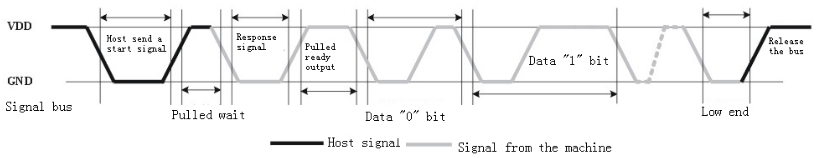
\includegraphics[width=12cm]{dht11_datagramm.png}
    \caption{Datagramm DHT-11 Sensor[1]}
    \end{center}
\end{figure}

\newpage
Ein Datagramm hat insgesamt 40 Bit und besteht aus:
\begin{itemize}
    \item 8 Bit Feuchtigkeitswert (Dezimal)
    \item 8 Bit Feuchtigkeitswert (Komma)
    \item 8 Bit Temperaturwert (Dezimal)
    \item 8 Bit Temperaturwert (Komma)
    \item 8 Bit Paritätsbit
\end{itemize}

Hier nun eine Beispielrechnung:

$$ % Mathematischer Block
\frac{0001 0100}{Luftfeuchtigkeit} + \frac{0000 0000}{Nachk.Luftf.}
 + \frac{0100 0101}{Temperatur} + \frac{0000 0000}{Nachk.Temp}
 = \frac{0101 1001}{Paritätsbit}
$$
\\
Die Empfangen Daten sind Korrekt da die Summe das \textbf{Paritätsbit} ergeben!
\\\\
Hierbei sind die Übertragenen Werte\ldots\\
\textbf{Luftfeuchtigkeit}: 0001 0100, 0000 0000 = 14,0H = 20,0\%\\
\textbf{Temperatur}: 0100 0101, 0000 0000 = 45,0H = 69°C 

\begin{figure}[h]
    \begin{center}
        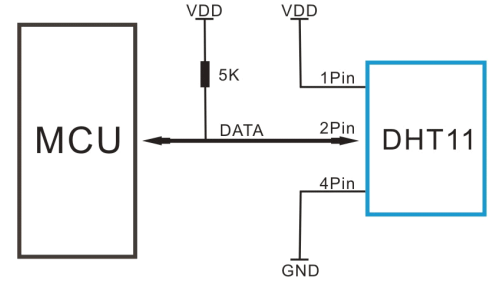
\includegraphics[width=4cm]{dht11_schem.png}
    \caption{DHT-11 Anschlussplan[2]}
    \end{center}
\end{figure}

\newpage
\subsection{MQ-2 (Gasdetektierung)}
Mit dem MQ-2 Sensor lässt sich die Luftqualität beziehungsweise die
Menge an bestimmten Gasen (Einheit: \textbf{PPM} - Parts Per Million) in der Luft.
Diese bestimmten Gase sind: Wasserstoff, Kolbenstoffmonoxid, \textbf{Rauch} und
noch weitere\ldots\\
\\
Zu demonstrationszwecken wurde \textbf{Rauch} ausgewählt. Das Prinzip zum Messen
einer Gaskonzentration ist aber bei allen gleich.
Da der Sensor über den Analogeingang mit einer Auflösung von 10 Bit
betrieben wird und dadurch `nur' Werte von 0 bis 1023 eingelesen werden, bedarf
es einer Berechnung um auf die PPM Werte von Rauch in der Luft zu kommen.
Hinzuzufügen ist noch, das der Sensor, um möglichst genau messen zu können, für
24h bei sauberer Luft betrieben werden muss. Im inneren des Sensors befindet
sich eine Heizspule welchen den Sensor auf die spezifizierte Temperatur bringen
soll.

\begin{figure}[h]
    \begin{center}
        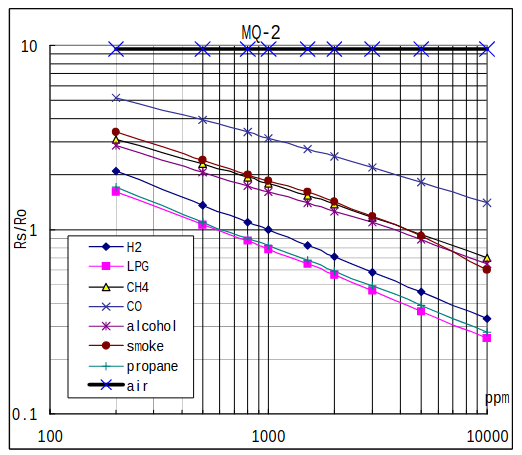
\includegraphics[width=9cm]{mq2_log.png}
    \caption{Logarithmische Skala des MQ-2[3]}
    \end{center}
\end{figure}

Auf der Y-Achse wird der Messwiderstand Rs eines bestimmten Gases dargestellt.
Während Ro der Messwiderstand bei sauberer Luft ist. Auf der X-Achse Sieht man
die PPM.
\newpage
Um die Steigung der Kurve bei einer logarithmischen Skala näherungsweise zu
berechnen, betrachten wir die braune Kurve und fügen die Werte aus dem
Schaubild in diese Formel ein:

$$
slope = \frac{Y_{2}-Y_{1}}{X_{2}-X_{1}}
$$
$$
slope = \frac{\log(0,5)-\log(3,5)}{\log(10000)-\log(200)}
$$
\texttt{smoke\_curve = [X1, Y1, slope]}\\
\texttt{curve\_curve = [2.301, 0.554, -0.497]}

\begin{figure}[h]
    \begin{center}
        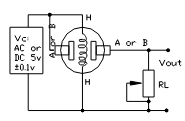
\includegraphics[width=5cm]{mq2_schem.png}
    \caption{MQ-2 Schaltung[4]}
    \end{center}
\end{figure}

Um bei der Messung des Sensors möglichst genau zu sein, ist es notwendig den
Sensor vor beginn der Datenerfassung zu kalibrieren, bzw. seinen Widerstand Ro 
bei sauberer Luft zu berechnen. 

\subsection{MQTT}
Wie bereits erwähnt wird die MQTT Architektur zum veröffentlichen der Nachrichten
im Netzwerk genutzt. Es handelt sich hierbei um eine \textbf{publish-subscribe}
Architektur. Der Client kommuniziert hier nicht direkt mit einem Server, sondern
mit einer middleware, dem \textbf{Broker}, welcher die Nachrichten nur an
den Client ausliefert wenn dieser ein bestimmtes Toppic \textbf{`abonniert`}
hat.\\

In diesem Fall ist der Publisher der ESP8266. Dieser veröffentlicht Daten auf
den Topics: `\texttt{/wetterstation/temperature}`, `\texttt{/wetterstation/humidity}`
und `\texttt{/wetterstation/smoke}`.\\

Die Payload der Nachrichten ist bei MQTT ein oder mehrere Strings beziehungsweise
Strings die mit JSON encoded sind.
\newpage
\subsection{Programmablauf}

Mit den Informationen zur Durchführung im Hinterkopf ergibt folgende
Vorgehensweise:

\begin{figure}[h]
    \begin{center}
        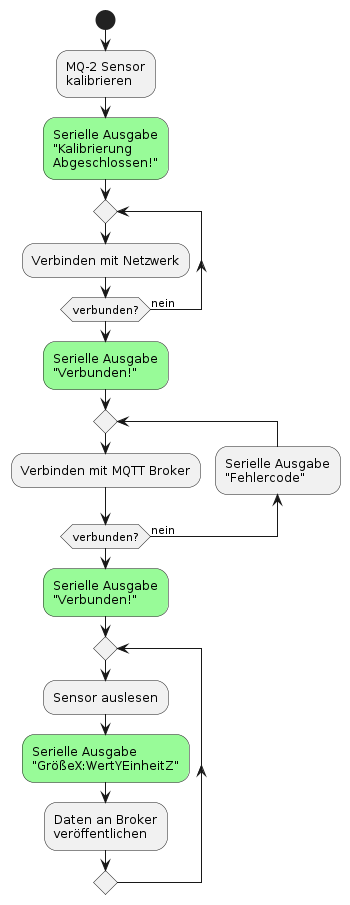
\includegraphics[width=5.5cm]{activity_system.png}
    \caption{Aktivitätsdiagramm Wetterstation}
    \end{center}
\end{figure}

\newpage
\section{Durchführung}
\subsection{DHT-11 Codeblock}
Zum Auslesen der Werte für \textbf{Temperatur} und \textbf{Luftfeuchtigkeit}
wurden die Programmbibliotheken \texttt{<DHT.h>}, \texttt{<DHT\_U.h>} \&
\texttt{<Adafruit\_Sensor.h>} verwendet.
\\\\
Programmatisch wurde das Auslesen der Sensorwerte wie folgt durchgeführt...
\\\\
\textbf{Temperatur}:
\begin{lstlisting}[language=C, style=code]
...
  if (isnan(event.temperature)) {
    Serial.println(F("Error reading temperature!"));
  }
  else {
    Serial.print(F("Temperature: "));
    Serial.print(event.temperature);
...
\end{lstlisting}
Fast gleich, hier aber nicht aufgeführt ist der Codeblock für die 
\textbf{Luftfeuchtigkeit}.

\subsection{MQ-2 Codeblock}

Um plausible Daten für die Rauchmessung zu erhalten, muss der MQ-2 Sensor
an sauberer Luft kalibriert werden. Es wird das Arithmetische Mittel von Ro
berechnet:

\begin{lstlisting}[language=C, style=code]
...
  for(int i = 0; i < 20; i++) {
    val += mqResistanceCalc(analogRead(MQPIN));
    Serial.print(F("."));
    delay(500);
  }
  val = val / 20;
  val = val / CLEAN_AIR_FACTOR;
...
\end{lstlisting}

Berechnung von Ro:

\begin{lstlisting}[language=C, style=code]
...
float mqResistanceCalc(int adc){
  return(((float)RL_VALUE*(1023/adc)/adc));
}
...
\end{lstlisting}
\newpage
Wert von Rs bestimmen:

\begin{lstlisting}[language=C, style=code]
void mqRead(){
...
  float rs = 0;
  for(int i = 0; i < 5; i++){ 
    rs += mqResistanceCalc(analogRead(MQPIN));
    delay(50);
  }
  rs = rs / 5;
...
\end{lstlisting}

Verhältniss von Rs zu Ro berechnen und die in Abschnitt 1.2 berechnete
`Rauchkurve' als Parameter an Annäherungsfunktion übergeben:

\begin{lstlisting}[language=C, style=code]
...
void mqRead(){
...
  float rs_ro_ratio = rs / ro;
  ppm = smokeLogScale(rs_ro_ratio, smoke_curve);
...
\end{lstlisting}

Berechnung des `Rauchwerts' in PPM:

\begin{lstlisting}[language=C, style=code]
int smokeLogScale(float ratio, float* curve){
  return pow(10, (((log(ratio) - curve[1]) / curve[2])
         + curve[0]));
}
\end{lstlisting}

\subsection{String Formatting für MQTT Message Publishing}
Es wurde bererits im Kapitel MQTT darauf eingegangen, dass Nachrichten als Strings
veröffentlicht werden. Da die gemessenen Werte aber andere Datentypen sind,
müssen diese erst in einem String repräsentiert werden. Die Vorgehensweise
ist bei bei allen drei Sensoren identisch. Daher nur ein Beispiel:

\begin{lstlisting}[language=C, style=code]
...
  ppm = smokeLogScale(rs_ro_ratio, smoke_curve);
  ...          
  sprintf(ppm_str, "%d", ppm);  // String Formatting                     
  const char* ppm_cstr = ppm_str;
  client.publish("/wetterstation/smoke", ppm_cstr);
...
\end{lstlisting}

Die letzte Zeile des vorherigen Codeblocks zeigt wie die Payload veröffentlicht
wird (Ebenfalls identisch zum Rest).

\subsection{MQTT Konfiguration}
Der Broker muss um Nachrichten zu Empfangen, gestartet und Konfiguriert werden.
Das ist über verschiedene Wege möglich. Es gibt MQTT Service Anbieter im
Internet. Diese kann man für Tests verwenden, man sollte aber vorsichtig sein,
da die Daten öffentlich für jeden Subscriber sind, der auf dem Topic zuhört.

\newpage
Alternativ dazu können MQTT Broker auch als Deamon unter einem Betriebssystem
oder in einem Docker Container gestartet werden. Smarthome Systeme wie Homeassistant
erlauben es auch MQTT Broker zu integrieren und diese als Addon laufen zu lassen.
In diesem Fall wird Mosquitto als Homeassistant Addon verwendet.

\subsubsection{Publisher}
Wetterstation benötigt um auf dem Broker zu veröffentlichen
Benutzer und Zugriffsrechte.
Angenommen die Daten sind vorhanden, so werden diese in die unter
\texttt{`wetterstation/src/mqtt\_config.h`} als Werte zu den Entsprechenden
Variablen eingetragen:

\begin{lstlisting}[language=C, style=code]
const char* mqtt_server = "<Broker IP Adresse>";
const int mqtt_port = 1883; // Standart Port
const char* mqtt_user = "<Benutzername MQTT-User>";
const char* mqtt_password = "<Passwort MQTT-Broker>";
\end{lstlisting}

\subsubsection{Subscriber}
Der Subscriber kann ein beliebiger client sein. Als Beispiel wird hier ein
Server verwendet. In der Konfiguration des Servers müssen ebenfalls Benutzer und
Zugriffsdaten hinterlegt werden. Natürlich müssen diese auch Vorhanden sein.
In Homeassistant unter \texttt{`configuration.yaml`} können diese eintragen werden:

\begin{lstlisting}[language=C, style=code]
...
mqtt:
  broker: <Adresse des Brokers>
  username: "<username>"
  password: "<password>"
  sensor:
    - name: "<freien Namen vergeben>"
      state_topic: "/wetterstation/humidity"
      unit_of_measurement: "%"
    ...
\end{lstlisting}

\section{Resultat}
Das Projekt konnte erfolgreich beendet werden. Es ist gelungen Messgrößen von
(digital \& analog) einzulesen und diese in einem Netzwerk zu weiteren
verarbeitung zu veröffentlichen. Durch die Grundlagen die durch dieses Projekt
geschaffen wurden, können nun jegliche Anwendungsfälle bezogen auf MQTT und
Sensoren in angriff genommen werden.
Folgend noch ein paar Bilder zur erfolgreichen Integration in die Smarthome
Anwendung.

\begin{figure}[h]
    \begin{center}
        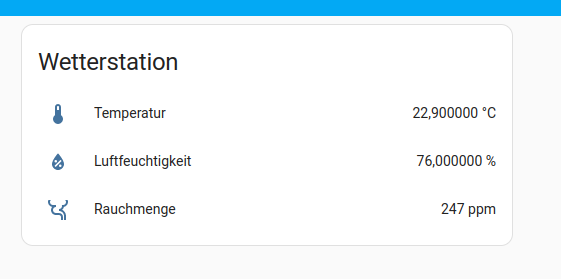
\includegraphics[width=12cm]{sm_card.png}
        \caption{Karte mit allen Senorwerten (Rauchtest)}
    \end{center}
\end{figure}

\begin{figure}[h]
    \begin{center}
        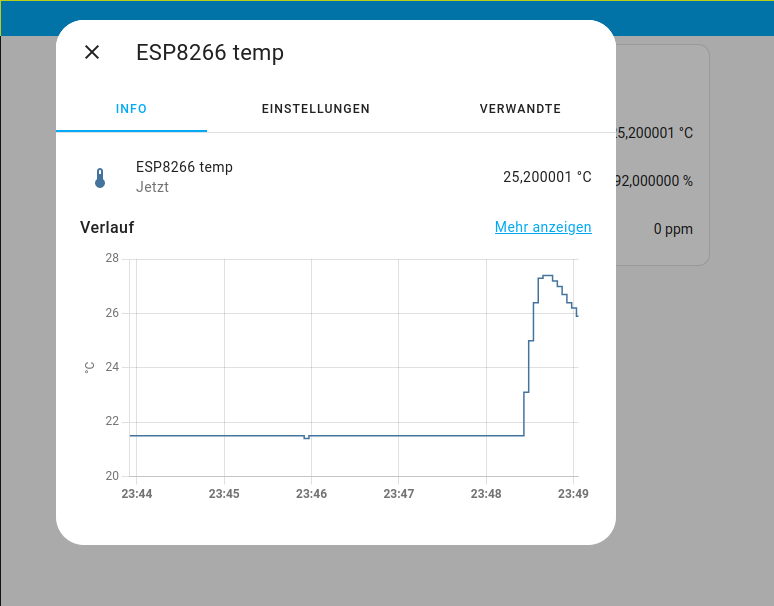
\includegraphics[width=12cm]{temp_hist.png}
    \caption{Verlauf Temperatur}
    \end{center}
\end{figure}

\clearpage

\section{Quellen}

Prof. Dr. Frankhauser, Thomas.\href{https://fankhauser.io/topics/mqtt/}{MQTT}. Abgerufen am: 13.01.2023.
[3]Unbekannt. \href{http://sandboxelectronics.com/files/SEN-000004/MQ-2.pdf}{Datasheet MQ-2}. Abgerufen am: 13.01.2023.
Das, Debashis. \href{https://circuitdigest.com/microcontroller-projects/interfacing-mq2-gas-sensor-with-arduino}{How Does MQ-2 Flammable Gas and Smoke Sensor Work with Arduino?}. Abgerufen am: 13.01.2023.
Unbekannt. \href{https://www.survivingwithandroid.com/esp8266-mqtt-client-publish-subscribe/}{ESP8266 MQTT Client: Publish and Subscribe Node-RED Dashboard}. Abgerufen am: 13.01.2023.
[1]Unbekannt. \href{https://components101.com/sites/default/files/component_datasheet/DHT11-Temperature-Sensor.pdf}{DHT11 Product Manual}. Abgerufen am: 13.01.2023.
[2]Unbekannt. \href{https://components101.com/sites/default/files/inline-images/Circuit-using-DHT11%E2%80%93Temperature-Sensor.png}{Connection Diagramm}. Abgerufen am: 13.01.2023.
[4]Gupta, Sourav, \href{https://circuitdigest.com/sites/default/files/inlineimages/u2/MQ6-Gas-Sensor-Pinout_0.png}{Gas Detection and PPM Measurement using PIC Microcontroller and MQ Gas Sensors}. Abgerufen am: 13.01.2023.

\end{document}
